\documentclass{article}
\usepackage{amsmath,amssymb}%添加数学宏包
\usepackage{graphics}
\usepackage{grffile}
\usepackage{CTEX}
\usepackage{parskip}
\begin{document}
\title{etherlab}
\author{221501029潘泓旭}
\date{221501029@smail.nju.edu.cn}
\maketitle
\noindent
%插入图片

1.  b4:8c:9d:50:59:c3\\
2.  10:51:72:1b:24:9f,不是,它是路由器的地址\\
\begin{figure}[htbp]
    \centering
    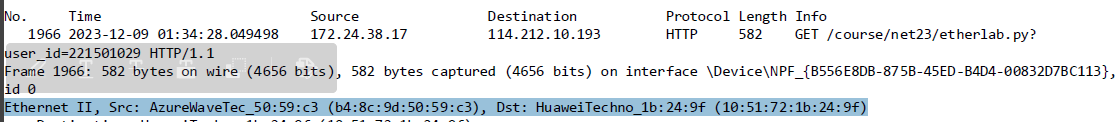
\includegraphics[width=1\textwidth]{pic/p1.png} % 图片文件名和路径
\end{figure}

3.  0x800;IP协议\\
\begin{figure}[htbp]
    \centering
    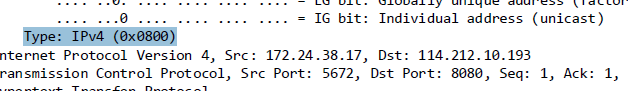
\includegraphics[width=1\textwidth]{pic/p2.png} % 图片文件名和路径
\end{figure}

4.  55\\
\begin{figure}[htbp]
    \centering
    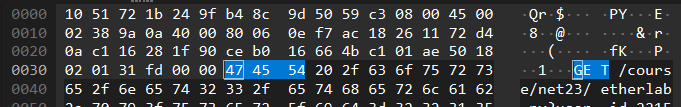
\includegraphics[width=1\textwidth]{pic/p3.png} % 图片文件名和路径
\end{figure}
\newpage
5.10:51:72:1b:24:9f,都不是,是我路由器的地址,是用来进我子网的链路\\
6.b4:8c:9d:50:59:c3,是\\
7.0x800,IP协议\\

\begin{figure}[htbp]
    \centering
    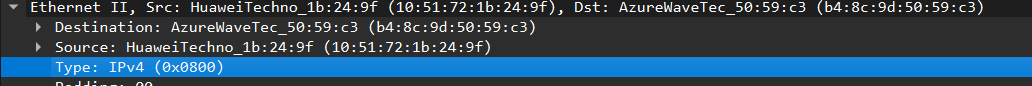
\includegraphics[width=1\textwidth]{pic/p5.png} % 图片文件名和路径
\end{figure}

8.有13个字节\\
\begin{figure}[htbp]
    \centering
    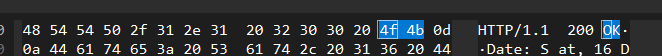
\includegraphics[width=1\textwidth]{pic/p6.png} % 图片文件名和路径
\end{figure}

9.Internet地址,物理地址,类型\\
\begin{figure}[htbp]
    \centering
    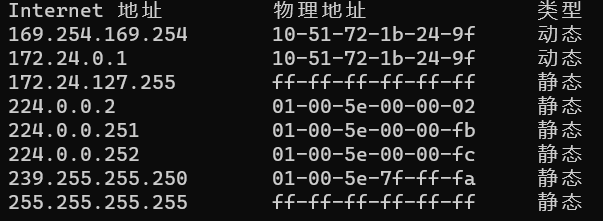
\includegraphics[width=1\textwidth]{pic/p7.png} % 图片文件名和路径
\end{figure}
\newpage
10.源地址是b4:8c:9d:50:59:c3,目的地址是ff:ff:ff:ff:ff:ff\\
11.0x0806,ARP协议\\
\begin{figure}[htbp]
    \centering
    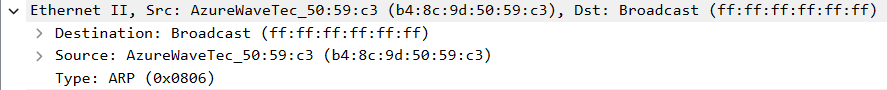
\includegraphics[width=1\textwidth]{pic/new1.png} % 图片文件名和路径
\end{figure}

12.a)20\\
   b)0x0001\\
   c)包含\\
   d)设置Target Mac address为00:00:00:00:00:00,Target IP address为192.168.168.162
\begin{figure}[htbp]
    \centering
    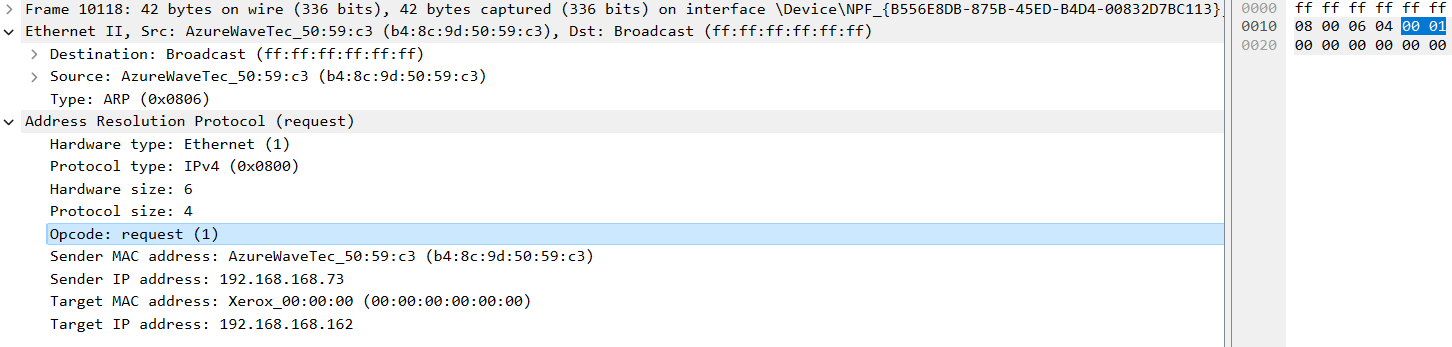
\includegraphics[width=1\textwidth]{pic/new2.png} % 图片文件名和路径
\end{figure}

13.a)20\\
   b)0x0002\\
   c)Sender MAC address为16:4f:9e:20:ba:ef,Target IP address为192.168.168.162\\

14.源地址为16:4f:9e:20:ba:ef,目的地址为b4:8c:9d:50:59:c3\\
\begin{figure}[htbp]
    \centering
    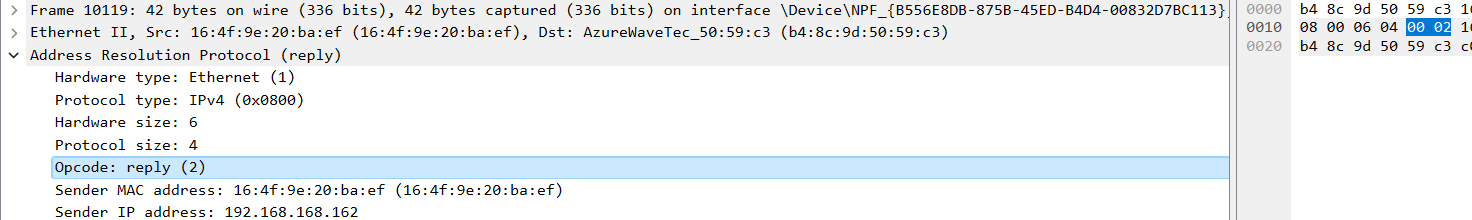
\includegraphics[width=1\textwidth]{pic/new3.png} % 图片文件名和路径
\end{figure}
\newpage
15.因为 ARP 广播信息是广播的,所有该网段内的电脑均可收到,而 ARP 广播回复是单播的,只有请求的那台电脑才能收到,因此抓不到另外一台电脑的 ARP 请求。\\
\begin{figure}[htbp]
    \centering
    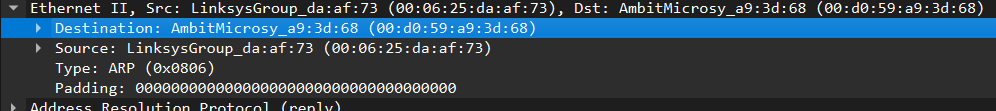
\includegraphics[width=1\textwidth]{pic/new4.png} % 图片文件名和路径
\end{figure}

EX1.会显示"ARP 项添加失败: 拒绝访问。"\\

\begin{figure}[htbp]
    \centering
    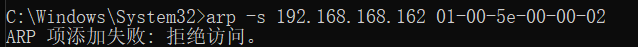
\includegraphics[width=1\textwidth]{pic/ex2.png} % 图片文件名和路径
\end{figure}

EX2. 根据微软官方文档http://support.microsoft.com/kb/949589,并没有ARP缓存保留默认时间\\
\end{document}